\documentclass{article}

\usepackage{ragged2e}
\usepackage{graphicx}
\usepackage{amsmath}
\usepackage{siunitx}
\usepackage{hyperref}

\renewcommand{\c}[1]{\texttt{#1}}

\begin{document}

%\begin{flushright}
    \noindent
    Rodrigo Becerril Ferreyra\\
    CECS 346 Section 03\\
    Lab 2\\
    Date: 17 September 2020
%\end{flushright}

\section{Introduction} The purpose of this lab is
twofold: the first objective is to practice
connecting external peripherals (devices such as switches
and LEDs) to the TM4C123G Evaluation Kit Board
(``LaunchPad'' or ``board''),
and the second objective is to program the board to implement a
simple program that flashes or toggles LEDs according to
user input via switches.

\section{Hardware} Although both software and hardware was
designed and implemented concurrently, the hardware was the
easiest part. One issue I had is the fact that the switches
that I own are too big to fit inside breadboard holes that
accommodate \num{22} gauge wire. Instead, I used a
male-to-female dupont wire, forced the switch's pins
into the female side, and used the male side to plug into
the breadboard. Other than that, the hardware building was
straightforward.

\section{Software} The software was the trickiest part.
Using the datasheet, I was quickly able to find the base
registers for Ports B and E, and fill the blanks in.
I copied most of the initialization function from Lab 1:
Hello LaunchPad, modifying values whenever necessary. Before
I got started on the logic to switch or flash the lights,
I tested all three ports individually to see if the lights
were hooked up properly, and to see if not too much current
was flowing through the LED and therefore the board (if
too much current
was passing through the board, I would have set the
appropriate register(s)
(\c{GPIODR2R}, \c{GPIODR4R}, or \c{GPIODR8R})). After
verifying the connections, it was not much longer
until I had a working program. I had some difficulties
here and there with connections, like thinking a switch was
connected properly when it wasn't, but other than that,
everything went smoothly.

\pagebreak

\section{Media} \begin{itemize}
    \item Link to YouTube video of demonstration: \url{https://youtu.be/AT8ybO28zSw}
    \item Schematic diagram: \begin{figure}[h]
        \centering
        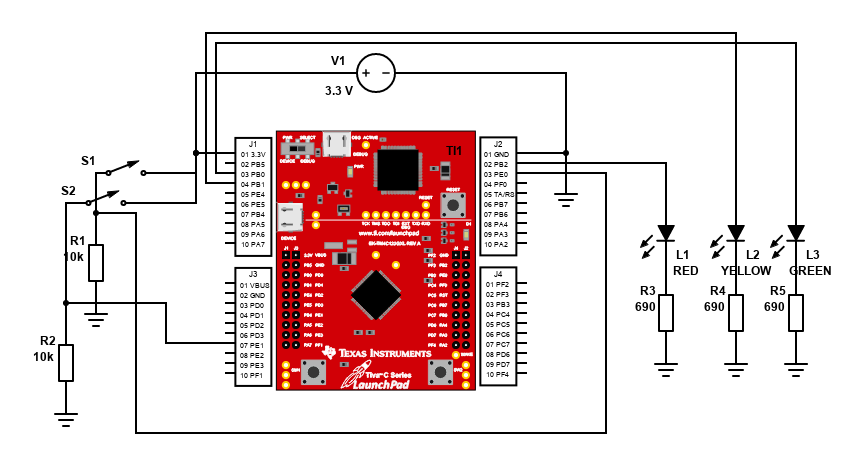
\includegraphics[width=\textwidth]{Images/schemeit-project.png}
        \caption{Schematic of project.}
        \label{fig1}
    \end{figure}
    \item Picture of hardware: \begin{figure}[h]
        \centering
        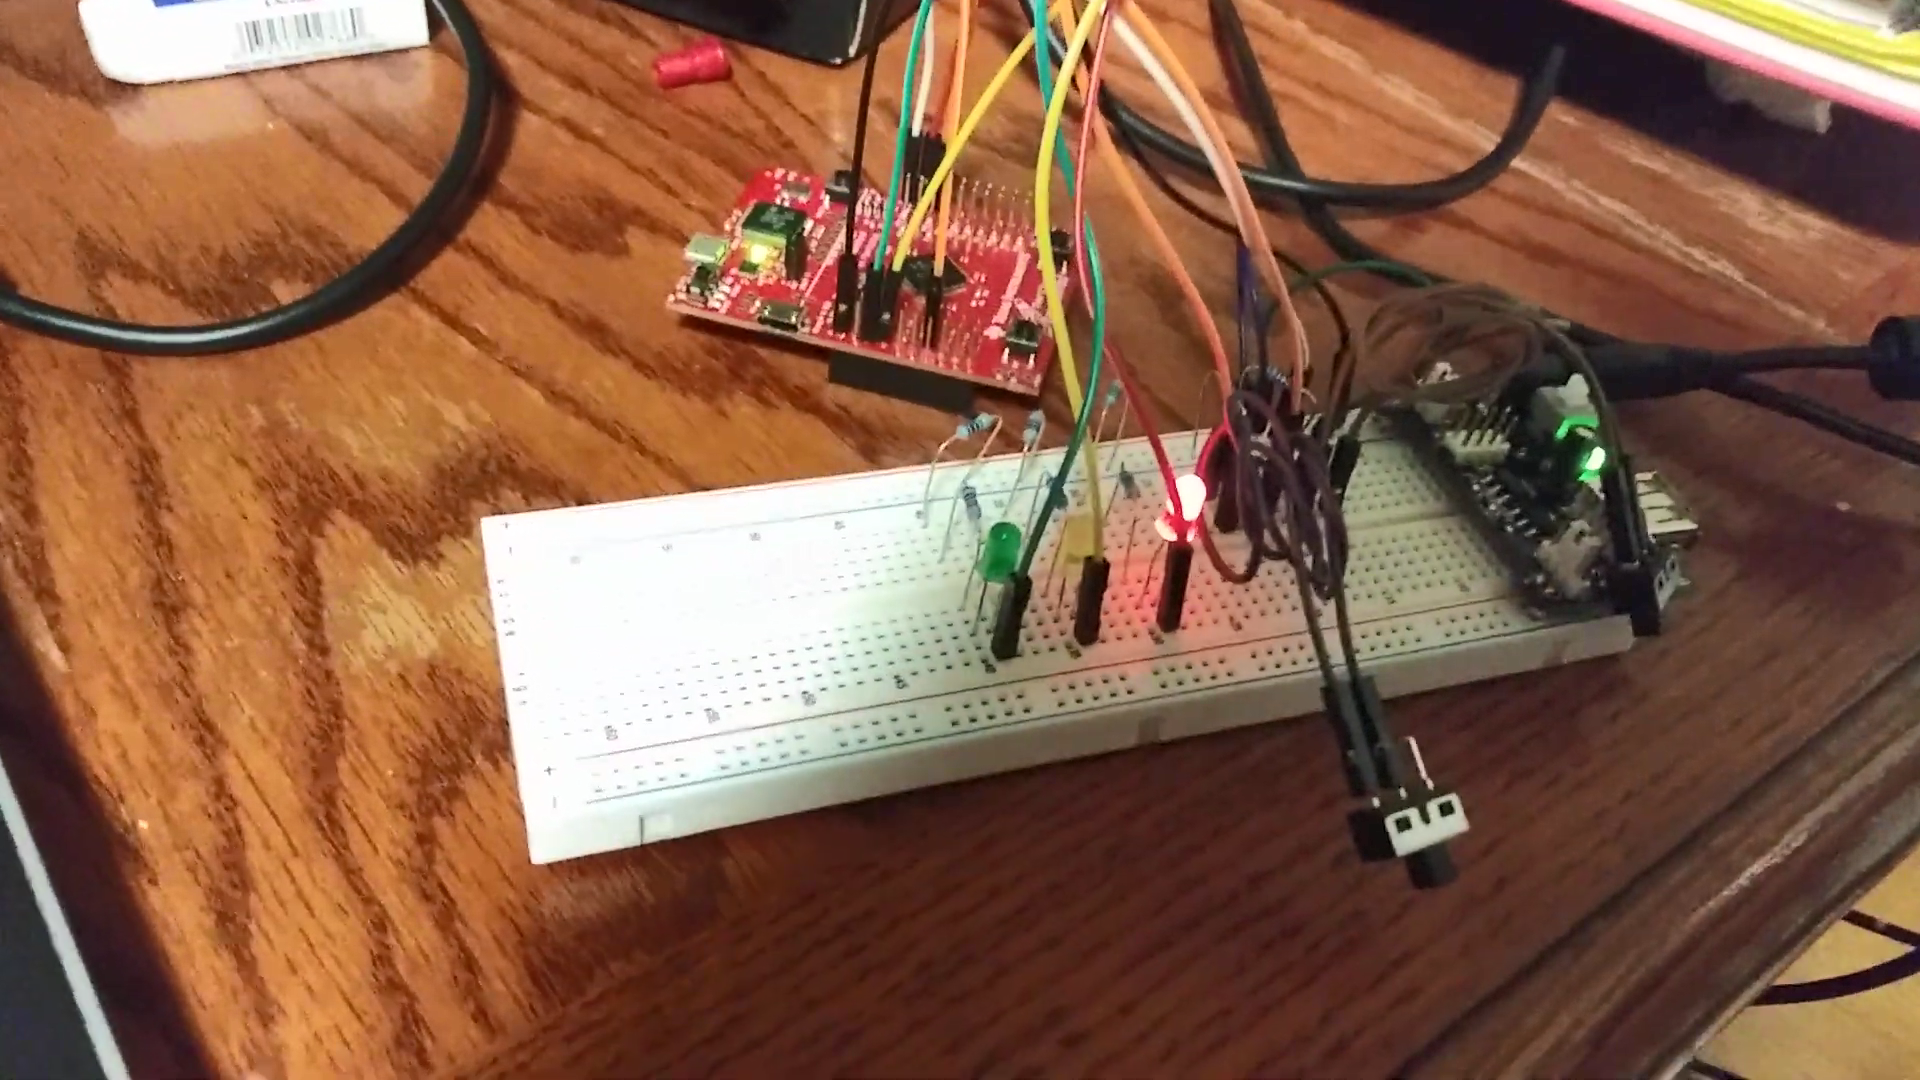
\includegraphics[height=170pt]{Images/workspace.png}
        \caption{Hardware running on breadboard with LaunchPad in the background.}
        \label{fig2}
    \end{figure}
\end{itemize}

\end{document}
